\documentclass[tikz,border=3pt]{standalone}
\usepackage{amsmath}
\usepackage{tikz}
\usetikzlibrary{shapes.geometric,arrows.meta,patterns,calc,decorations.pathreplacing}

\begin{document}
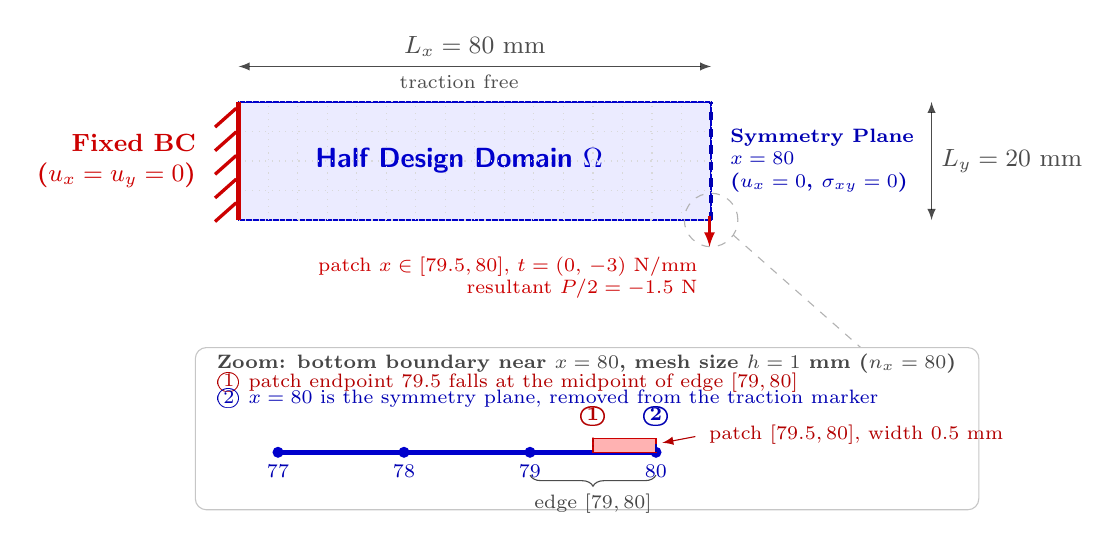
\begin{tikzpicture}[scale=1.0, >=latex]
  % FixedFixedBeamHalfDomain2d: 左半域 80 x 20 mm, 绘图比例 0.075 -> 6.0 x 1.5
  % 载荷区 x in [79.5, 80] 只有 0.5 mm 宽, 主图画不出, 细节见下方放大图。

  % ---------------- 主图 ----------------
  \draw[thick, fill=blue!8, draw=blue!80!black] (0,0) rectangle (6,1.5);
  \node[font=\bfseries\sffamily, color=blue!80!black] at (2.8,0.75) {Half Design Domain $\Omega$};

  \draw[step=0.375, gray!30, dotted] (0,0) grid (6,1.5);

  % Fully clamped Left Boundary (x = 0)
  \draw[ultra thick, red!80!black] (0,0) -- (0,1.5);
  \foreach \y in {0.1, 0.4, 0.7, 1.0, 1.3} {
    \draw[line width=1.2pt, red!80!black] (-0.3, \y-0.12) -- (-0.03, \y+0.12);
  }
  \node[left, red!80!black, font=\small\bfseries, align=right] at (-0.42,0.75)
    {Fixed BC\\($u_x = u_y = 0$)};

  % Symmetry Plane at x = 80
  \draw[ultra thick, blue!70!black, dashed] (6,0) -- (6,1.5);
  \node[right, blue!70!black, font=\scriptsize\bfseries, align=left] at (6.12,0.75)
    {Symmetry Plane\\$x = 80$\\($u_x = 0$, $\sigma_{xy} = 0$)};

  % Load patch on the bottom edge, x in [79.5, 80] (0.5 mm -> 0.0375, 主图不可见)
  \draw[line width=3pt, red!80!black] (5.96,0) -- (6.0,0);
  \draw[->, thick, red!80!black] (5.98,-0.04) -- (5.98,-0.34);
  \node[below left, red!80!black, font=\scriptsize, align=right] at (5.95,-0.34)
    {patch $x \in [79.5, 80]$, $t = (0,\,-3)$ N/mm\\resultant $P/2 = -1.5$ N};

  % Traction-free remainder
  \node[above, gray!60!black, font=\scriptsize] at (2.8,1.55) {traction free};

  % Dimensions
  \draw[<->, opacity=0.7] (0,1.95) -- (6,1.95) node[midway, above, font=\small] {$L_x = 80\text{ mm}$};
  \draw[<->, opacity=0.7] (8.8,0) -- (8.8,1.5) node[midway, right, font=\small] {$L_y = 20\text{ mm}$};

  % 放大标记
  \draw[gray!60, dashed] (6,0) circle (0.34);
  \draw[gray!60, dashed] (6.28,-0.19) -- (7.9,-1.62);

  % ---------------- 放大图: 底边 x in [77, 80], h = 1 mm ----------------
  % 映射 x_code -> 0.5 + 1.6*(x_code - 77): 77->0.5, 78->2.1, 79->3.7, 79.5->4.5, 80->5.3
  \draw[rounded corners=4pt, gray!45] (-0.55,-3.68) rectangle (9.4,-1.62);
  \node[right, gray!55!black, font=\scriptsize\bfseries] at (-0.4,-1.82)
    {Zoom: bottom boundary near $x = 80$, mesh size $h = 1$ mm ($n_x = 80$)};

  % 编号说明
  \node[right, font=\scriptsize, align=left, red!70!black] at (-0.4,-2.06)
    {\textcircled{1} patch endpoint $79.5$ falls at the midpoint of edge $[79,80]$};
  \node[right, font=\scriptsize, align=left, blue!70!black] at (-0.4,-2.28)
    {\textcircled{2} $x = 80$ is the symmetry plane, removed from the traction marker};

  % 边界线与网格节点 (节点号标在线下方)
  \draw[ultra thick, blue!80!black] (0.5,-2.95) -- (5.3,-2.95);
  \foreach \x/\lab in {0.5/77, 2.1/78, 3.7/79, 5.3/80} {
    \fill[blue!80!black] (\x,-2.95) circle (2.0pt);
    \node[below, font=\scriptsize, blue!70!black] at (\x,-2.99) {$\lab$};
  }

  % 载荷区 [79.5, 80] (画在线上方)
  \fill[red!30] (4.5,-2.95) rectangle (5.3,-2.77);
  \draw[red!80!black] (4.5,-2.95) rectangle (5.3,-2.77);
  \node[right, font=\scriptsize, red!70!black] at (5.85,-2.72) {patch $[79.5, 80]$, width $0.5$ mm};
  \draw[->, red!70!black] (5.80,-2.75) -- (5.38,-2.83);

  % 标记一: 载荷区左端落在边中点
  \draw[thick, red!70!black, densely dotted] (4.5,-2.95) -- (4.5,-2.76);
  \node[above, font=\scriptsize\bfseries, red!70!black] at (4.5,-2.74) {\textcircled{1}};

  % 标记二: 对称面被 marker 挖除
  \draw[thick, blue!70!black, dashed] (5.3,-2.95) -- (5.3,-2.76);
  \node[above, font=\scriptsize\bfseries, blue!70!black] at (5.3,-2.74) {\textcircled{2}};

  % 边 [79, 80] 的括注 (放在节点号下方)
  \draw[decorate, decoration={brace, mirror, amplitude=4pt}, gray!60!black]
    (3.7,-3.24) -- (5.3,-3.24);
  \node[below, font=\scriptsize, gray!55!black] at (4.5,-3.36) {edge $[79,80]$};
\end{tikzpicture}
\end{document}
